% ============================================================================
% CSCE 763: Digital Image Processing - Midterm Exam (Fall 2022)
% ============================================================================

\documentclass[12pt]{article}

% ============================================================================
% PACKAGE IMPORTS
% ============================================================================
\usepackage{amsmath}
\usepackage{graphicx}
\usepackage{amssymb}
\usepackage{tikz}
\usepackage[margin=1in]{geometry}
\usepackage{setspace}
\usepackage{xcolor}
\usepackage{enumitem}
\usepackage{tcolorbox}
\usepackage{fancyhdr}
\usepackage{booktabs}
\usepackage{array}
\usepackage{colortbl}
\usepackage{float}

% ============================================================================
% HEADER AND FOOTER SETUP
% ============================================================================
\pagestyle{fancy}
\setlength{\headheight}{14.5pt}
\fancyhf{}

\fancyhead[L]{Fall 2022}
\fancyhead[R]{CSCE 763: Digital Image Processing}

\renewcommand{\headrulewidth}{0pt}

% ============================================================================
% TIKZ LIBRARIES
% ============================================================================
\usetikzlibrary{shapes.geometric, arrows.meta, positioning, patterns, calc}

% --- USC Brand Colors ---
\definecolor{USC_Garnet}{HTML}{73000A}
\definecolor{USC_Sandstorm}{HTML}{FFF2E3}
\definecolor{USC_Black90}{HTML}{363636}
\definecolor{USC_Black70}{HTML}{5C5C5C}
\definecolor{USC_Black50}{HTML}{A2A2A2}
\definecolor{USC_Black10}{HTML}{ECECEC}
\definecolor{USC_Honeycomb}{HTML}{65780B}
\definecolor{USC_Atlantic}{HTML}{466A9F}
\definecolor{USC_Congaree}{HTML}{1F414D}
\definecolor{USC_Rose}{HTML}{CC2E40}

% ============================================================================
% CUSTOM COLORED BOXES
% ============================================================================
\newtcolorbox{stepbox}[1][Step]{
  colback=white,
  colframe=USC_Garnet,
  fonttitle=\bfseries,
  title=#1,
  sharp corners,
  colbacktitle=USC_Garnet,
  coltitle=white,
}

\newtcolorbox{resultsbox}{
  colback=white,
  colframe=USC_Honeycomb,
  fonttitle=\bfseries,
  title=Results,
  sharp corners,
  colbacktitle=USC_Honeycomb,
  coltitle=white,
}

% ============================================================================
% CUSTOM QUESTION COMMANDS
% ============================================================================
\newcommand{\problem}[1]{%
  \vspace{0.5cm}
  {\noindent\normalsize \textbf{#1}}
  \vspace{0.3cm}
}

% ============================================================================
% DOCUMENT INFORMATION
% ============================================================================

\title{\textbf{Midterm Exam}}
\author{}
\date{10/11/2022}

% ============================================================================
% BEGIN DOCUMENT
% ============================================================================

\begin{document}

\maketitle
\thispagestyle{fancy}
\setlength{\parindent}{0pt}

\setlist[enumerate,1]{label=\alph*)}
\setlist[enumerate,2]{label=(\roman*)}

% ============================================================================
% PROBLEM 1
% ============================================================================

\problem{Problem 1 part 1)}

Given the image region as shown in Figure 1 and $V = \{1\}$, what is the shortest m-path between $p$
(the pixel at the upper-left corner) and $q$ (the pixel at the bottom-right corner)? Give the length of
the path if the path exists. (15 points)

\begin{center}
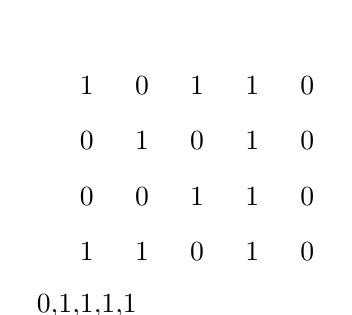
\begin{tikzpicture}[scale=0.7]
\foreach \y [count=\row from 0] in {
    {1,0,1,1,0},
    {0,1,0,1,0},
    {0,0,1,1,0},
    {1,1,0,1,0},
    {0,1,1,1,1}
} {
    \foreach \x [count=\col from 0] in \y {
        \node at (\col, -\row) {\x};
    }
}
\end{tikzpicture}
\end{center}

\vspace{2cm}

\problem{Problem 1 part 2)}

To take a picture for fireworks at night, give at least two operations that should be applied to
improve the visualization quality of the image and explain. (15 points)

\newpage

% ============================================================================
% PROBLEM 2
% ============================================================================

\problem{Problem 2)}

A, B, C and D are four sets. Give expressions for the set shown shaded in Figure 2 in terms of A,
B, C, and D. Note that all of the shaded areas constitute of one set

\begin{center}
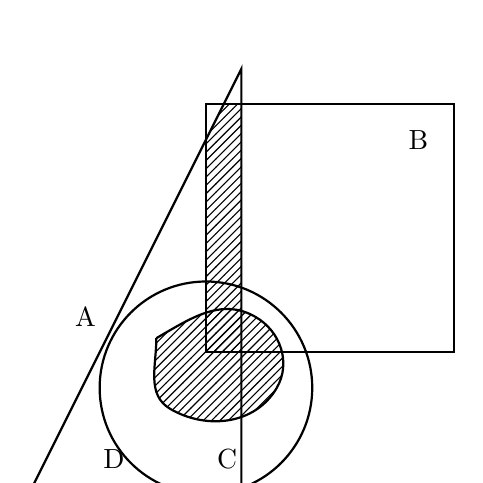
\begin{tikzpicture}[scale=0.9]
    % Define the shapes
    % A - Triangle
    \coordinate (A1) at (0,0);
    \coordinate (A2) at (3,6);
    \coordinate (A3) at (3,0);

    % B - Rectangle
    \coordinate (B1) at (2.5,2);
    \coordinate (B2) at (6,2);
    \coordinate (B3) at (6,5.5);
    \coordinate (B4) at (2.5,5.5);

    % C - Circle
    \coordinate (Ccenter) at (2.5,1.5);

    % D - Small ellipse/shape at bottom of triangle
    \coordinate (Dcenter) at (1.5,1);

    % Draw the shapes with pattern for shaded region
    % First fill the intersection region (simplified representation)
    \begin{scope}
        \clip (A1) -- (A2) -- (A3) -- cycle;
        \clip (B1) rectangle (B3);
        \fill[pattern=north east lines] (0,0) rectangle (6,6);
    \end{scope}

    % Draw outlines
    \draw[thick] (A1) -- (A2) -- (A3) -- cycle;
    \node at (0.8,2.5) {A};

    \draw[thick] (B1) rectangle (B3);
    \node at (5.5,5) {B};

    \draw[thick] (Ccenter) circle (1.5cm);
    \node at (1.2,0.5) {D};
    \node at (2.8,0.5) {C};

    % Small inner shape representing the complex intersection
    \draw[thick] (1.8,2.2) to[out=30,in=150] (3.2,2.5) to[out=-30,in=60] (3.5,1.5)
                 to[out=240,in=-30] (2,1.2) to[out=150,in=-90] (1.8,2.2);
    \fill[pattern=north east lines] (1.8,2.2) to[out=30,in=150] (3.2,2.5) to[out=-30,in=60] (3.5,1.5)
                 to[out=240,in=-30] (2,1.2) to[out=150,in=-90] (1.8,2.2);
\end{tikzpicture}
\end{center}

\newpage

% ============================================================================
% PROBLEM 3
% ============================================================================

\problem{Problem 3)}

Given a 3x3 spatial filter $\displaystyle\frac{1}{9}\begin{bmatrix} -1 & -1 & -1 \\ -1 & -17 & -1 \\ -1 & -1 & -1 \end{bmatrix}$ answer the following questions:

\begin{enumerate}
\item What type of filter is it? When applying this filter on an image, what kind of effect you
will expect in the output image? Why? (Hint: is this filter an image smoothing filter, an
image sharpening filter or an edge detector?) (10 points)

\item Perform the image convolution using this filter on a 3x3 image $\begin{bmatrix} 3 & 5 & 12 \\ 7 & 18 & 11 \\ 5 & 9 & 15 \end{bmatrix}$. Give the
CROPPED filtering result for the output image. (Hint: you need to assume an appropriate
zero mapping) (15 points)
\end{enumerate}

\newpage

% ============================================================================
% PROBLEM 4
% ============================================================================

\problem{Problem 4)}

An image with intensities in the range $r \in [0, L-1]$ has the pdf

\[
p_r(r) = \begin{cases} \displaystyle\frac{4r}{3(L-1)^2} & 0 \le r \le L-1 \\[0.5em] 0 & \text{otherwise} \end{cases}
\]

where $L-1$ is the maximum intensity value. It is desired to transform the intensity levels of this image so that they will have the specified pdf

\[
p_z(z) = \begin{cases} \displaystyle\frac{2z}{(L-1)^2} & 0 \le z \le L-1 \\[0.5em] 0 & \text{otherwise} \end{cases}
\]

Assume that the intensity value is continuous and find the transformation function $z = T(r)$ in terms of $r$ and $z$ that will accomplish this. (25 points)

\vspace{0.5cm}

(Hints: The transformation function of histogram equalization is given as

\[
s = T(r) = (L-1) \int_0^r p_r(w)\,dw
\]
)

\newpage

% ============================================================================
% BONUS QUESTION
% ============================================================================

\begin{center}
\textbf{Bonus Question}
\end{center}

Perform the Fourier transform to a function as shown in Figure 3. (20 points)

\vspace{0.3cm}

(Hint: the definition of the Fourier transform of a function is $\displaystyle F(u) = \int_{-\infty}^{\infty} f(t) e^{-j2\pi ut}\,dt$ )

\begin{center}
\begin{tikzpicture}[scale=0.8]
    % Axes
    \draw[->] (-4,0) -- (5,0) node[right] {$t$};
    \draw[->] (0,-0.5) -- (0,4.5) node[above] {$f(t)$};

    % Tick marks on x-axis
    \foreach \x in {-3,-2,-1,1,2,3,4} {
        \draw (\x,0.1) -- (\x,-0.1) node[below] {$\x$};
    }
    \node[below] at (0,-0.1) {$0$};

    % Tick marks on y-axis
    \foreach \y in {1,2,3} {
        \draw (0.1,\y) -- (-0.1,\y) node[left] {$\y$};
    }

    % The step function
    % From -3 to -2: height 1
    \draw[thick] (-3,0) -- (-3,1) -- (-2,1);
    % From -2 to -1: height 2
    \draw[thick] (-2,1) -- (-2,2) -- (-1,2);
    % From -1 to 0: height 3
    \draw[thick] (-1,2) -- (-1,3) -- (0,3);
    % From 0 to 1: height 3
    \draw[thick] (0,3) -- (1,3);
    % From 1 to 2: height 2
    \draw[thick] (1,3) -- (1,2) -- (2,2);
    % From 2 to 3: height 1
    \draw[thick] (2,2) -- (2,1) -- (3,1);
    % From 3 to 4: height 0
    \draw[thick] (3,1) -- (3,0) -- (4,0);
    % Before -3
    \draw[thick] (-4,0) -- (-3,0);
\end{tikzpicture}
\end{center}

% ============================================================================
% END OF DOCUMENT
% ============================================================================

\end{document}
